\documentclass[main.tex]{subfiles}
\begin{document}

\marginpar{Friday\\ 2022-1-14}

\subsubsection{The effect of a finite source size}

We take our usual picture with the upstream and downstream in one dimension; we take a certain \(x_0 \) in the upstream (so \(x_0 < 0\))
such that when a particle reaches it it completely leaves the system. 

\todo[inline]{Why does he draw the exponential as concave?}

We know that the solution is exponential, and it satisfies 
%
\begin{align}
D \eval{\pdv{f}{x}}_{1} = u_1 f_0 
\,.
\end{align}

We suppose that particles are leaving the surface at \(x_0 \) with 
a flux \(f_* c / 2 \approx u_1 f_0 \), 
therefore \(f_* \approx 2 (u_1 / c) f_0 \ll f_0  \).

The free escape boundary condition is \(f (x_0 ,p) =0 \). 

The equation we want to solve, in a stationary situation, is always 
%
\begin{align}
u \pdv{f}{x} &= \pdv{}{x} \left(  D \pdv{f}{x}\right)
+ \frac{1}{3} \dv{u}{x} p \dv{f}{p} + Q
\,,
\end{align}
%
and we have already seen that 
%
\begin{align}
\eval{\pdv{f}{x} }_{2} = 0
\,,
\end{align}
%
since in the downstream the solution must be constant. 

On the other hand, in the upstream 
%
\begin{align}
u \pdv{f}{x} = \pdv{}{x} \left( D \pdv{f}{x} \right)
\implies uf - D \pdv{f}{x} = \text{constant}
\,.
\end{align}

We now write the flux as 
%
\begin{align}
f = A \exp(\alpha x) + B
\,,
\end{align}
%
imposing our conditions: they tell us that 
%
\begin{align}
u_1  A \exp(\alpha x) + u_1 B - D A \alpha \exp(\alpha x) = k
\,,
\end{align}
%
therefore \(\alpha = u_1 / D\) and \(B = k / u_1\). 

The solution then reads 
%
\begin{align}
f = A \exp(\frac{u_1 x }{D}) + \frac{k}{u_1 }
\,,
\end{align}
%
but we also have 
%
\begin{align}
f(x= 0) &= A + k / u_1  \\
f(x = x_0 )&= A \exp(\frac{u_1 x_0 }{D}) + \frac{k}{u_1 } = 0
\,.
\end{align}

Subtracting these, we get 
%
\begin{align}
A (1 - \exp(\frac{u_1 x_0 }{D})) = f_0 
\,,
\end{align}
%
while 
%
\begin{align}
\frac{k}{u_1 } = - \frac{\exp(u_1 x_0 / D)}{1 - \exp(u_1 x_0 / D)}
\,.
\end{align}

The full solution then reads 
%
\begin{align}
f(x, p) &= \frac{f_0}{1 - \exp(u_1 x_0 / D)}  \left(\exp( \frac{u_1 x}{D} ) - \exp( \frac{u_1 x_0 }{D}) \right)
- 
\,.
\end{align}

The strategy is always to join these solutions at the boundary:
integrating the solution there yields 
%
\begin{align}
D \eval{\pdv{f}{x}}_{2} - D \eval{\pdv{f}{x}}_{1}
+ \frac{1}{3} (u_2 - u_1 ) p \pdv{f}{p} = 0
\,,
\end{align}
%
but the derivative of the distribution function evaluated at \(0^-\) is 
%
\begin{align} 
D \eval{\pdv{f}{x}}_{1} = \frac{f_0}{1 - \exp(u_1 x_0 / D)} u_1 
\,,
\end{align}
%
and we can approximate the exponential as 
%
\begin{align}
\exp( \frac{u_1 x_0 }{D}) \approx 1 + \frac{u_1 x_0 }{D}
\,,
\end{align}
%
as long as the particles are leaving the system at a distance which is small compared to the diffusion length scale. 
The opposite limit, \(\abs{x_0 } \gg u_1 / D\), is the one in which we retrieve the situation we discussed previously. 

Note that both of these could be included in the same system, since \(D\) depends on the particle momentum! 

We can reframe the equation as 
%
\begin{align}
\frac{ \dd{f_0 }}{f_0 } &= \frac{ \dd{p}}{p} \frac{3 u_1 }{u_2 - u_1 }
\frac{1}{1 - \exp(u_1 x_0 / D)}
\,.
\end{align}

The solution is therefore 
%
\begin{align}
f_0 (p) \propto \exp(
    \int_{p _{\text{min}}}^{p}
    \frac{ \dd{p'}}{p'} \frac{3 u_1 }{u_2 - u_1 }
\frac{1}{1 - \exp(u_1 x_0 / D)}
)
\,.
\end{align}

There  is a momentum \(p_*\) such that \(\abs{x_0} = D(p_*) / u_1  \). 

If \(p \ll p_*\), we get \(D/u_1 \ll \abs{x_0 }\), so the exponential is of a large negative quantity, meaning we can neglect it and find
%
\begin{align}
f_0 (p) \propto \left( \frac{p}{p _{\text{min}}}\right)^{-3 \frac{u_1}{u_1 - u_2 }}
\,.
\end{align}

This is the usual solution. 

On the other hand, if \(p \gg p_*\) we get the exponential of a quantity close to zero, which we can expand:
%
\begin{align}
f_0 (p) \sim \left(\frac{p_*}{p _{\text{min}}}\right)^{-3r / (r-1)}
\exp(- \int_{p_*}^{p} \frac{ \dd{p'}}{p'} \frac{3 u_1 }{u_1 - u_2 } \frac{D}{u_1 \abs{x_0 }})
\,.
\end{align}

At a momentum close to \(p_*\), we get an exponential suppression with respect to the powerlaw! 
The integrand in the big negative exponential is large (as the exponential \(\exp(u_1 x_0 / D)\) is close to 1). 

When particles have enough momentum to reach the ``leaving surface'', they simply leave! 

\begin{extracontent}
Exercise: take the derivative of the distribution function at \(x = x_0 \). Then, at \(p\) very small compared to \(p_*\), the escaping flux goes to zero. 
On the other hand, at very large \(p\) the flux also goes to zero! 
\end{extracontent}

This means that only particles with momentum very close to \(p_*\) leave! 
We get a peaked flux!
Since \(f\) is zero there, we will only have the \(D \pdv*{f}{x}\) term.

We also want to know how broad the distribution is. 

In real systems, \(u_1\) is not constant: it slows down in time, selecting lower and lower energies, and the peak at \(p_*\) is moving left. 
In the end, even though at a given time the spectrum is peaked, if we integrate over the size of the system a spectrum is still found. 

We are approaching the problem that the accelerated particles are producing their own magnetic field, but far enough from the shock there will be few particles and the ones which reach this length will be able to leave. 

\begin{extracontent}
A second exercise: what if we impose the boundary condition that \(f(x_0, p)\) is not zero, but instead it equals the (small) background cosmic ray density in the galaxy? 

The PDE system to solve is 
%
\begin{align}
u_1 \pdv{f}{x} &= \pdv{}{x} \left( D \pdv{f}{x} \right)  \\
D \eval{\pdv{f}{x}}_{x=0^{-}} &= \frac{1}{3} (u_2 - u_1 ) p \eval{\pdv{f}{p}}_{x=0^{-}}  \\
f(x= x_0) &= g(p) = A \left( \frac{p}{p _{\text{min}}} \right)^{- \alpha  _{\text{CR}}}
\,.
\end{align}
%

Let us assume the solution looks like 
%
\begin{align}
f(x, p) \propto \exp(\frac{x u_1 }{D}) \left(\frac{p}{p _{\text{min}}}\right)^{- \beta (x)}
\,,
\end{align}
%
and for convenience let us define the characteristic diffusion wavenumber \(k = u_1 / D\). 

Then, the first equation upstream tells us that 
%
\begin{align}
(\beta ')^2 = \beta '' + k \beta '
\,,
\end{align}
%
while the condition at the shock tells us that 
%
\begin{align}
\left( k - \beta '\right) =  \frac{1}{3} \frac{r - 1 }{r} k \beta 
\,.
\end{align}

Finally, the condition at the \(x_0 \) border tells us that 
%
\begin{align}
\beta (x = x_0 ) = \alpha _{\text{CR}}
\,,
\end{align}
%
a fixed number.

The solution is basically as follows: when \(D / u_1 \ll \abs{x_0 }\) the spectral index \(\beta (x = 0)\) is basically \(3r/(r-1)\), while when \(D / u_1 \gg \abs{x_0 }\) the spectral index at \(x=0\) is basically the same as the one at \(x_0 \). 

So, on a rough level in momentum space we expect a broken powerlaw spectrum, with index \(3r/(r-1)\) at low momenta and index \(\alpha _{\text{CR}}\) at high momenta, where the two are separated at \(p_*\) such that \(D(p_*) = u_1 \abs{x_0 }\). 

Let us solve the ODE for \(\beta \) explicitly, with respect to the variable \(X = kx\): the ansatz
%
\begin{align}
\beta (X) = -\log (c_1 e^{X} + 1) + X + c_2 
\,,
\end{align}
%
works, since \(\beta ' = -c_1 e^X /(c_1 e^X + 1) + 1\) 
and \(\beta '' = +c_1^2 e^{2X} / (c_1 e^X + 1)^2 - c_1 e^X / (c_1 e^X + 1) \), therefore 
%
\begin{align}
(\beta ')^2 - \beta '' &= \frac{c_1^2 e^{2X}}{(c_1 e^X + 1)^2} - 2 \frac{c_1 e^X}{c_1 e^X + 1} + 1  - \frac{c_1^2 e^{2X}}{(c_1 e^X + 1)^2} + \frac{c_1 e^X}{c_1 e^X + 1} \\
&= - \frac{c_1 e^X}{(c_1 e^X + 1)} + 1 = \beta '
\,.
\end{align}

The boundary conditions will fix \(c_1 \) and \(c_2 \): 
at \(x = x_0 \), meaning \(X= X_0 = x_0 u_1 / D \), we have \(\beta = \alpha _{\text{CR}}\), so 
%
\begin{align}
\alpha _{\text{CR}} = - \log (c_1 e^{X_0}  + 1) + X_0  + c_2
\,.
\end{align}

At \(X =0 \), on the other hand, we get 
%
\begin{align}
1 - \beta ' = \frac{c_1 e^X}{c_1 e^X + 1} &= \frac{1}{3} \frac{r-1}{r} \left( - \log \left( c_1 e^X + 1\right) + X + c_2  \right)  \\
\frac{c_1 }{c_1 + 1} &= \frac{1}{3} \frac{r-1}{r} \left( - \log (c_1 + 1) + c_2  \right)
\,.
\end{align}

Maybe we do not need to solve the whole thing: the combination we really need is 
%
\begin{align}
\beta_0 = \beta (X = 0) = - \log (c_1 + 1) + c_2 
\,,
\end{align}
%
so we have 
%
\begin{align}
\beta_0 &= \frac{3r}{r-1} \frac{c_1 }{c_1 + 1}  \\
c_2 &= + \log (c_1 e^{X_0} + 1) - 1 + \alpha _{\text{CR}} \\
\beta_0 &= - \log (c_1 + 1 ) + c_2  \\
&= \log \frac{c_1 e^{X_0} + 1}{c_1 + 1} - X_0  + \alpha _{\text{CR}}
\,.
\end{align}

This also means we can make an equation for \(c_1 \) alone! 
%
\begin{align}
c_2 &= \frac{3r}{r-1} \frac{c_1}{c_1 + 1} + \log(c_1 + 1)  \\
&= + \log (c_1 e^{X_0} + 1) - 1 + \alpha _{\text{CR}}  \\
\alpha _{\text{CR}} &= + \frac{3r}{r-1} \frac{c_1}{c_1 + 1} + \log(c_1 + 1) - \log (c_1 e^{X_0} + 1) + X_0   \\
&= \underbrace{\frac{3r}{r-1} \frac{c_1}{c_1 + 1}}_{\beta_0 } + \log \frac{c_1 + 1}{c_1 + e^{-X_0 }}
\,.
\end{align}

Notice that an admissible solution, as long as \(\alpha _{\text{CR}} = 3r/(r-1)\), is \(\beta = \text{const}\). 
This corresponds to the \(c_1 \to \infty\) limit, where also \(c_2 = \alpha _{\text{CR}}\).

Now we are basically done! If we are given \(X_0 \) and \(\alpha _{\text{CR}}\) we can compute \(\beta_0\). 
\end{extracontent}

\begin{figure}[ht]
\centering
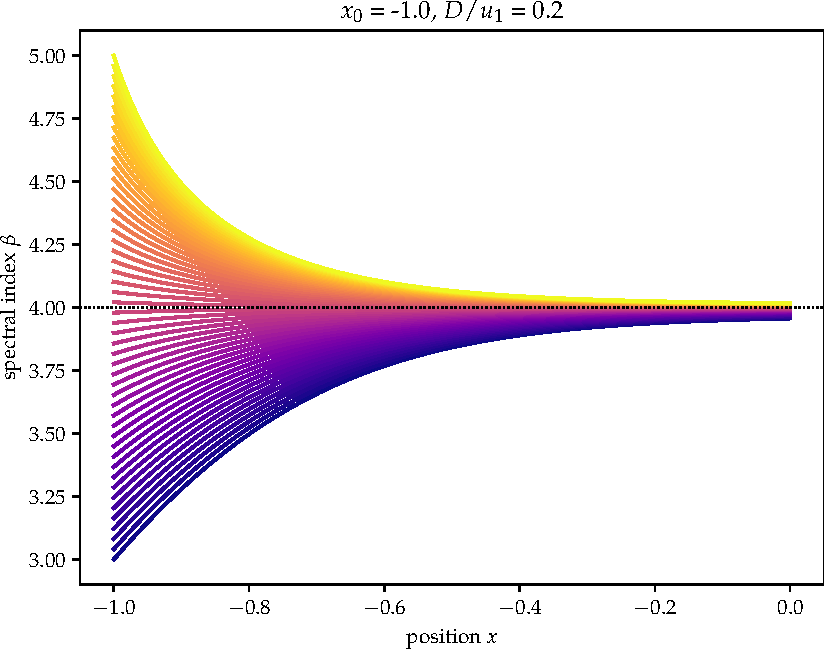
\includegraphics[width=\textwidth]{figures/cosmic_ray_reacceleration_far}
\caption{Reacceleration with \(D/u_1 \ll \abs{x_0 }\).}
\label{fig:cosmic_ray_reacceleration_far}
\end{figure}

\begin{figure}[ht]
\centering
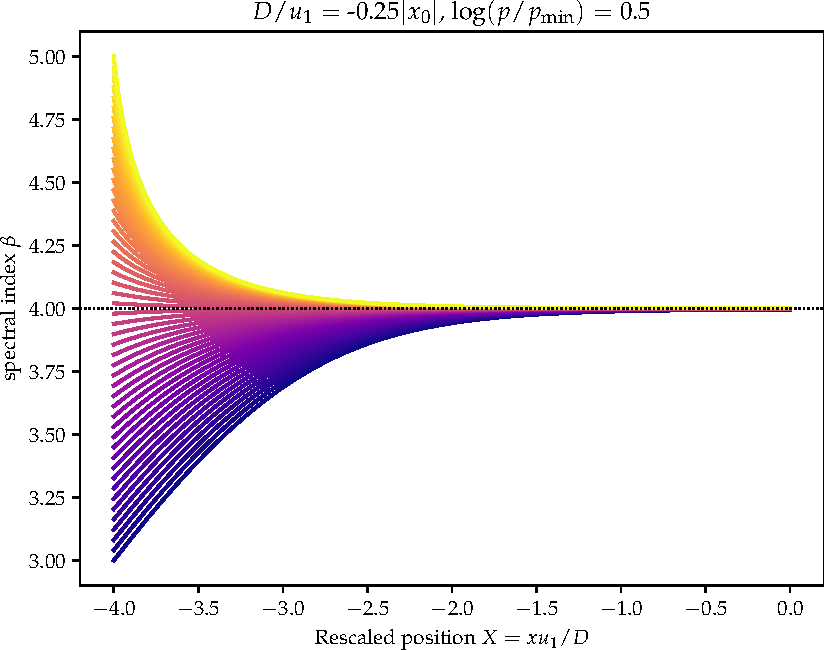
\includegraphics[width=\textwidth]{figures/cosmic_ray_reacceleration_near}
\caption{Reacceleration with \(D/u_1 \gg \abs{x_0 }\).}
\label{fig:cosmic_ray_reacceleration_near}
\end{figure}

We will get an interesting phenomenon: \emph{reacceleration}. 
Particles from the galaxy are pushed up in energy. 

We suppose to have a powerlaw spectrum: 
%
\begin{align}
f(x = x_0 , p) = A (p / p _{\text{min}})^{-\alpha }
\,,
\end{align}
%
with the two cases of \(\alpha \) being smaller or larger than \(3r / (r-1)\). 

We now want to give an estimate of the \emph{acceleration time}: 
this is useful since we typically have information about the age 
of the systems which may produce cosmic rays. 

The proper way would be to start from the transport equation, 
and move to a Laplace transform. 

We then still join solutions at the boundary as usual; 
we then take the limit as \(s \to 0\), which corresponds to infinite time. 

This is very instructive: we find a decreasing exponential in time, 
in the form of \(\exp(-t / \tau )\), where \(\tau \) is the acceleration time. 
This will also yield a formal answer as to why the derivative of the distribution downstream must vanish.

\begin{extracontent}
We are welcome to try to do this exercise.
\end{extracontent}

We will derive the acceleration time in a simpler way. 

If the cosmic rays have a density \(n _{\text{CR}}\), and supposing the flux per unit area is \(\Sigma \), ??? will be 

\todo[inline]{what? what is this quantity?}
%
\begin{align}
\frac{n_{\text{CR}} v}{4} \Sigma \tau_1 = \frac{n _{\text{CR}} \Sigma D }{u_1 }
\,.
\end{align}

Therefore, 
%
\begin{align}
\tau_1 = 4 \frac{D}{u_1 v} 
\,,
\end{align}
%
and we can do the same thing downstream, which yields \(\tau_2 = 4 D_2 / v u_2 \). 

The total timescale is therefore \(\tau = \tau_1 + \tau_2 \). 

We also know that 
%
\begin{align}
\frac{\Delta E}{E }= \frac{4}{3} \frac{u_1 - u_2 }{v }
\,,
\end{align}
%
so 
%
\begin{align}
\tau _{\text{acc}} = \frac{E}{\dv{E}{t}} = \frac{E}{\Delta E} \Delta t = \frac{3}{4} \frac{v}{u_1 - u_2 } \frac{4}{v} \left( \frac{D}{u_1 } + \frac{D}{u_2 }\right)
\,,
\end{align}
%
therefore 
%
\begin{align}
\tau = \frac{3}{u_1 - u_2 } \left(
    \frac{D}{u_1 } + \frac{D}{u_2 }
\right)
\,,
\end{align}
%
while the Laplace transform approach yields 
%
\begin{align}
\tau _{\text{acc}} = \frac{3}{u_1 - u_2 } \int_{p _{\text{min}}}^{p} \frac{ \dd{p'}}{p'} \left(
    \frac{D}{u_1 } + \frac{D}{u_2 }
\right)
\,,
\end{align}
%
so, as an order of magnitude, \(\tau \sim D / u_1^2\). 

This expression tells us something important: even if \(D_2\) is small, since downstream there is a mess, we still need \(D_1 \) to be small as well in order for the acceleration timescale to allow for decent particle acceleration. 

We were always assuming that the particles were protons. 

Synchrotron emission scales like \(E^2\), so we cannot neglect it for electrons. 
Since electrons emit energy so fast, it is easier to see the effect of their acceleration. 

We need to modify the transport equation to account for energy losses, and we need a way to inject them. 

The temperature of the protons will be larger than the temperature of the electrons. 
The electrons will have much smaller Larmor radii, meaning that their injection will be harder. 

How to account for energy losses? 
%
\begin{align}
u \pdv{f}{x} = \pdv{}{x} \left( D \pdv{f}{x}\right) 
+ \frac{1}{3} \dv{u}{x} p \pdv{f}{p} + Q
- \frac{f}{\tau _{\text{losses}} (p) }
\,,
\end{align}
%
this term, known as ``catastrophic energy loss'', is not really accurate; the proper way to do it would be 
%
\begin{align}
\frac{1}{p^2} \pdv{}{p} \left(p^2 \dot{p} f\right)
\,,
\end{align}
%
but if we write it that way there is no analytic solution. 
If the spectrum is a powerlaw, these two formulation are close to each other. 

Let us integrate around the shock: the new term is continuous, so it integrates to zero and we get
%
\begin{align}
\eval{D \pdv{f}{x}}_{2} -
\eval{D \pdv{f}{x}}_{1} 
+ \frac{u_2 - u_1 }{3} p \pdv{f_0 }{p} 
\,.
\end{align}

Let us start by assuming that \(f\) is constant downstream; 
upstream on the other hand we have 
%
\begin{align}
\pdv{}{x} \left(
    u_1 f - D \pdv{f}{x} 
\right)
= - \fdv{f}{ \tau _{\text{loss}}(p)}
\,.
\end{align}

We can try to solve this with an exponential ansatz: 
%
\begin{align}
f &= A \exp( x / \lambda )  \\
\pdv{f}{x} &= \frac{A}{\lambda } \exp( \frac{x}{\lambda })
\,,
\end{align}
%
which yields 
%
\begin{align}
A \pdv{}{x} \left(
   \exp( \frac{x}{\lambda } ) - \frac{D}{\lambda } \exp( \frac{x}{\lambda }) 
\right) &= A \exp( \frac{x}{ \lambda })  \\
\frac{1}{\lambda } \left( u - \frac{D}{\lambda }\right) &= - \frac{1}{\tau _{\text{loss}}}  \\
\lambda u \tau  - D \tau  + \lambda^2 &= 0
\,.
\end{align}

This means we have 
%
\begin{align}
\lambda = \frac{- u_1 \tau + \sqrt{(u_1 \tau )^2 + 4 D \tau }}{2}
\,,
\end{align}
%
where we must choose the plus solution since \(\lambda \) must be positive, so that we get a decreasing exponential.

The boundary term reads 
%
\begin{align}
- D_1 \eval{\pdv{f}{x}}_{1} = - D_1 \frac{f_0}{\lambda } 
\,,
\end{align}
%
so we have 
%
\begin{align}
- D_1 \frac{f_0 }{\lambda } + \frac{u_2 - u_1 }{3} p \pdv{f_0 }{p} = 0
\,.
\end{align}

The terms in the square root we are comparing are: \((u \tau )^2\), 
the square of the distance the particles move over a loss time, 
and \(D \tau \), the square of the distance they diffuse over a loss time. 

Comparing these is equivalent to comparing 
%
\begin{align}
\frac{4 D}{u_1^2} = \tau _{\text{acc}} \lessgtr \tau _{\text{loss}}
\,.
\end{align}

Let us suppose that the acceleration timescale is indeed much smaller than the energy loss scale: 
then, we can approximate \(\lambda \)     as 
%
\begin{align}
\lambda &\approx u \frac{\tau}{2} \left(-1 + \sqrt{1 + \frac{4 D \tau }{(u \tau )^2}}\right)
 \\
&\approx \frac{u \tau }{2} \frac{2D \tau }{u^2 \tau } = \frac{2 D \tau }{u}
\,,
\end{align}
%
so the result is the same as the case without losses. 

What if, instead, the acceleration is slow compared to energy losses?
The scale \(\lambda \) will be 
%
\begin{align}
\lambda \approx \sqrt{D \tau }
\,.
\end{align}

This means that the particles are only getting as far from the shock as \(\sqrt{D \tau }\), not very far. 

In this case we get 
%
\begin{align}
f_0 \propto \exp( \int_{p _{\text{min}}}^{p} \frac{ \dd{p'}}{p'} \frac{3}{u_1 - u_2 } \frac{D_1}{\lambda (p)})
\,.
\end{align}

Now, we know that 
%
\begin{align}
\tau _{\text{loss}} \sim \frac{E}{ \Delta E / \Delta t} \sim \frac{E}{E^2} \sim \frac{1}{p}
\,,
\end{align}
%
while \(D / u^2\) is a growing function of \(p\)! 
We get two regimes! 
At low energies acceleration dominates, while at high energies losses start to dominate, and we get an exponential suppression of the spectrum as well. 

For Bond diffusion, we get a hard exponential since \(D \sim p\) while \(\lambda \sim 1/ p\): we get a suppression like \(\exp(- (p / p_*)^2 )\). 

We assumed \(\pdv*{f}{x} = 0\) downstream, but instead we can solve the equation like upstream now. 

Next time we will briefly look at the supernova remnant paradigm, but that is not the only possibility. 

We could do the same thing for protons, but we would get 
a much larger size than any concrete source. 

\end{document}